\documentclass{tufte-handout}

\usepackage{amsmath}
\usepackage{physics}
\usepackage{graphicx}
%nice tables
\usepackage{booktabs}
\usepackage{subfloat}

%use si units
\usepackage{siunitx}
\title{}
\author{Adam A. S. Green}
\date{}

\begin{document}

\bibliographystyle{plain}
\newcommand{\leo}[1]{Professor Leo Radzihovsky}

%make new phase commands to save having to right it out all the time.
\newcommand{\smapr}{$\mathrm{SmAP}_\mathrm{R}$}
\newcommand{\sma}{$\mathrm{SmA}$}
\newcommand{\smc}{$\mathrm{SmC}$}
\newcommand{\smapf}{$\mathrm{SmAP}_\mathrm{F}$}
\newcommand{\smapa}{$\mathrm{SmAP}_\mathrm{A}$}
\newcommand{\smcapalp}{$\mathrm{SmC}_\textrm{A}\textrm{P}_\mathrm{\alpha}$}
\newcommand{\smapalp}{$\mathrm{SmAP}_\mathrm{\alpha}$}
\newcommand{\smcapf}{$\mathrm{SmC}_\textrm{A}\textrm{P}_\mathrm{F}$}
\newcommand{\smcspf}{$\mathrm{SmC}_\textrm{S}\textrm{P}_\mathrm{F}$}
\newcommand{\smcspa}{$\mathrm{SmC}_\textrm{S}\textrm{P}_\mathrm{A}$}
\newcommand{\smcapa}{$\mathrm{SmC}_\textrm{A}\textrm{P}_\mathrm{A}$}
\newcommand{\smca}{$\mathrm{SmC}_\textrm{A}$}
\newcommand{\smcs}{$\mathrm{SmC}_\textrm{S}$}
\newcommand{\smcapaprime}{$\mathrm{SmC}_\textrm{A}\textrm{P}_\mathrm{A'}$}
%make new phase commands to save having to right it out all the time.
\newcommand{\smaprM}{\mathrm{SmAP}_\mathrm{R}}
\newcommand{\smaM}{\mathrm{SmA}}
\newcommand{\smapfM}{\mathrm{SmAP}_\mathrm{F}}
\newcommand{\smapaM}{\mathrm{SmAP}_\mathrm{A}}
\newcommand{\smapalpM}{\mathrm{SmAP}_\mathrm{\alpha}}
\newcommand{\smcapfM}{\mathrm{SmC}_\textrm{A}\textrm{P}_\mathrm{F}}
\newcommand{\smcspfM}{\mathrm{SmC}_\textrm{S}\textrm{P}_\mathrm{F}}
\newcommand{\smcspaM}{\mathrm{SmC}_\textrm{S}\textrm{P}_\mathrm{A}}
\newcommand{\smcapaM}{\mathrm{SmC}_\textrm{A}\textrm{P}_\mathrm{A}}

\newcommand{\smcsM}{\mathrm{SmC}_\textrm{S}}
\newcommand{\smcapaprimeM}{\mathrm{SmC}_\textrm{A}\textrm{P}_\mathrm{A`}}

\newcommand{\nsix}{\textbf{n-16}}
\newcommand{\nfour}{\textbf{PAL30}}
\maketitle

\begin{abstract}
\noindent 
Though \nfour{phi} has been well characterized by our study, there are several
open questions that remain for me--- some of which are specific to \nfour{phi},
and some of which are more general to the implications of the phases that we
discovered.
\end{abstract}
\section{Specific Questions}
\subsection{Polarization Current vs. Optical Tilt}
%include this figure

\begin{marginfigure}
    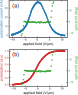
\includegraphics[width=\linewidth]{./figs/PRCvsTilt/T110.png}
    \caption{Polarization and optical tilt of \nfour{phi}. (a) The polarization
        current (PC) and the optical tilt. (b) The cumulative integral of the PC,
        $P(E) \propto \int_{E'=0}^{E'=E}dP/dE' dE'+A$, should be proportional to
        the total polarization, with offset $A$, plotted with the optical tilt.
    }
\end{marginfigure}

\subsection{Model for Polar Switching}
\subsection{Model for Helical Flucuations}
\subsection{Structure-property Relations} % looking at the homolog series
\section{General Questions}
\subsection{Onset of Chirality}
%Look at ferri phases of calamitics, they usually have the same phase sequence
\subsection{Bent-Core vs. Calamitic} % with regards to the formation of helices
\subsection{Point-Group Chirality vs Ensemble Chirality}

%\begin{marginfigure}
%    \includegraphics[width=\linewidth]{}
%    \caption{} 
%\end{marginfigure}
\end{document}
